%File: formatting-instruction.tex
\documentclass[letterpaper]{article}
\usepackage{aaai}
\usepackage{times}
\usepackage{helvet}
\usepackage{courier}
\usepackage{color}
\usepackage{textcomp}
\usepackage{amsthm}
\usepackage{amssymb}
\usepackage{amsmath}
\usepackage{graphicx}
\usepackage{xcolor}
\usepackage{comment}
\usepackage{xspace}

\newcommand{\argmin}{\operatornamewithlimits{argmin}}
\newcommand{\argmax}{\operatornamewithlimits{argmax}}
\newcommand{\bE}{\mathbb{E}}
\newcommand{\bx}{\mathbf{x}}
\newcommand{\bg}{\mathbf{g}}
\newcommand{\bu}{\mathbf{u}}
\newcommand{\bU}{\mathbf{U}}
\newcommand{\cI}{\mathcal{I}}
\newcommand{\cC}{\mathcal{C}}
\newcommand{\cQ}{\mathcal{Q}}
\newcommand{\tta}{\mathtt{a}}
\newcommand{\tth}{\mathtt{h}}
\newcommand{\ttz}{\mathtt{z}}
\newcommand{\PW}{\mbox{PW}}
\newcommand{\BR}{\mbox{BR}}
\newcommand{\defword}[1]{\textbf{\boldmath{#1}}}
\newcommand{\ie}{{\it i.e.}\xspace}
\newcommand{\eg}{{\it e.g.}\xspace}
\newtheorem{definition}{Definition}
\newtheorem{fact}{Fact}
\newtheorem{theorem}{Theorem}
\newtheorem{corollary}{Corollary}
\newtheorem{lemma}{Lemma}
\newtheorem{proposition}{Proposition}
\newcommand{\Proof}{{\noindent\bf Proof. }}
\newcommand{\citejustyear}[1]{\cite{#1}}
\newcommand{\Qed}{$\blacksquare$}
\newcommand{\abs}[1]{\left|#1\right|}
\newcommand{\todo}[1]{{\color{red}{\bf #1}}}

% the note center!
\definecolor{darkgreen}{RGB}{0,125,0}
\newcounter{vlNoteCounter}
\newcounter{mlNoteCounter}
\newcounter{asNoteCounter}
\newcommand{\vlnote}[1]{{\scriptsize \color{blue} $\blacksquare$ \refstepcounter{vlNoteCounter}\textsf{[VL]$_{\arabic{vlNoteCounter}}$:{#1}}}}
\newcommand{\mlnote}[1]{{\scriptsize \color{darkgreen} $\blacksquare$ \refstepcounter{mlNoteCounter}\textsf{[ML]$_{\arabic{mlNoteCounter}}$:{#1}}}}
\newcommand{\asnote}[1]{{\scriptsize \color{red} $\blacktriangle$ \refstepcounter{asNoteCounter}\textsf{[AS]$_{\arabic{asNoteCounter}}$:{#1}}}}
%\newcounter{NoteCounter}
%\newcommand{\vlnote}[1]{{\scriptsize \color{blue} \refstepcounter{vlNoteCounter}\textsf{[VL]$_{\arabic{vlNoteCounter}}$:{#1}}}}
%\renewcommand{\vlnote}[1]{}

\frenchspacing
\setlength{\pdfpagewidth}{8.5in}
\setlength{\pdfpageheight}{11in}
\pdfinfo{
/Title (Searching Imperfect Information Games using Online Counterfactual Regret Minimization)
/Author (Authors)}
\setcounter{secnumdepth}{0}  
 \begin{document}
% The file aaai.sty is the style file for AAAI Press 
% proceedings, working notes, and technical reports.
%
\title{Search in Imperfect Information Games using Online\\Counterfactual Regret Minimization}
\author{Authors}
%\author{Author info\\
%Association for the Advancement of Artificial Intelligence\\
%2275 East Bayshore Road, Suite 160\\
%Palo Alto, California 94303\\


\maketitle

\begin{abstract}
Online search in games has been a classic interest of artificial intelligence.
Advances made in search for perfect information games (such as Chess, Checkers, Go, and Backgammon) have led to AI capable of defeating the world's top human experts. 
The progress of search in imperfect information games (such as Poker, Bridge, and Skat) has comparatively lagged behind, due mainly to the complexities introduced by hidden information. 
In this paper, we present Online Outcome Sampling (OOS), the first imperfect information search algorithm with formal guarantees of convergence to an equilibrium strategy in a zero-sum game.   
In addition, we show that OOS avoids the common problems encountered by determinization.
We evaluate the practical performance and convergence rate of OOS and compare to two modern imperfect information search algorithms.
OOS is shown to outperform its competitors in randomly generated game trees as well as several complex domains: 
Dudo, Phantom Tic-Tac-Toe, and (a bigger one). 
\end{abstract}

\section{Introduction}

%Main points: 
%\begin{itemize}
%\item motivate importance of convergence to NE. 
%\item why online search vs. offline equilibrium computation
%\item existing methods may not converge over time (it would be great to have a motivating example that convinces the reader that any determinization-based II search algorithm cannot converge in general - some kind of search game could be a good example)
%\item introduce the first one that does, and show that it can compete with the others in practice
%\end{itemize}

In many sequential multi-agent interactions, the agents first have some initial time to prepare for the interaction and then after each decision, they have an additional thinking time to decide about their next move. When the preparation time is abundant and the computational resources sufficient, an equilibrium strategy for a smaller abstract game can be pre-computed and then used during the game play. This {\it offline approach} has been remarkably successful in Computer Poker \cite{}.
However, the preparation time is often very limited. The exact model of the game may become known only shortly before the play, such as in general game-playing, security enforcement in previously unknown environment, and general-purpose robotics. In a short time, only a very small abstract game could be solved in advance. Moreover, it might not even be possible to create a sufficiently small and still useful abstraction to be solved in time. In these cases, agents may need to {\it decide online}: make initial decisions quickly and then put additional effort to improving their strategy in the current situation while the interaction is taking place.

%Search in game-playing has been a classic interest of artificial intelligence. 
%focused on perfect information games, 
When restricted to perfect information settings, the field of online search has benefited from decades of research in game-playing. 
%as evidenced by events such as defeat of human chess champions, 
%solving of checkers, and the growing strength of computer Go programs~\cite{Campbell02deepblue,Schaeffer07gameover,Gelly12}.
Due to the complexity and problems introduced by hidden information, search in imperfect information settings has received comparatively much less attention.
%This is unfortunate as many sequential decision-making problems have some element of hidden information. 
Modern approaches to imperfect information search use different forms of {\it determinization} to sample possible states, then run 
searches rooted from these states, aggregating their results choose an action to play. The most extreme forms, Perfect Information Monte Carlo (PIMC)~\cite{Long10Understanding} ``averages over clairvoyance''~\cite{AIBook},
% ML-Note Nov2: @Viliam, PIMC *is* "averaging over clairvoyance"
ignore the information structure completely. While this is sufficient in some games, it does not work well in games like simplified (Kuhn) poker and 
Monte Carlo Tree Search (MCTS) applied to Kriegspiel~\cite{Ciancarini10Kriegspiel}. 
Following the success in Kriegspiel, most recent algorithms try to fix the problem by accounting for the information structure during the 
search in some way. These approaches seem to improve performance in Kriegspiel, Skat~\cite{Furtak13Recursive}, 
Scotland Yard~\cite{Nijssen12SY}, Dou Di Zhu, Magic: The Gathering, and other card games~\cite{Cowling12MTG,Cowling12ISMCTS}.

%For example, the notion of a subgame is required for backward induction, 
%which most perfect information search algorithms are based on, is not well-defined in imperfect information games. 

The main problem of the current techniques is a lack of theoretical foundations of the algorithms. There are no guarantees that the algorithms will always find a good strategy in a game, given a sufficient thinking time. In fact, there is practical evidence suggesting that some of these techniques will not converge to the optimal solution even in very small games like Biased Rock-Paper-Scissors and Kuhn poker~\cite{Shafiei09,Ponsen11Computing}.

In this paper, we start by formalizing the problem of imperfect information search from the ground up. That is, we return to the game-theoretic 
foundations upon which search in games is built to motivate the importance of Nash equilibrium as the optimal strategy in zero-sum games. We explain the subtleties introduced by imperfect information that cause the current approaches not to converge to the optimal strategy. We introduce Online Outcome Sampling (OOS), a simulation-based MCTS-like algorithm that builds its search tree incrementally. 
We formally prove that OOS converges to an equilibrium strategy as time increases, making it the first 
known imperfect information search algorithm satisfying this property, which we call {\it consistency}. Furthermore, we analyze methods for incorporating the information obtained by the players in the game to the search process, so that the consistency property is preserved. We show the empirical convergence rates and performance of OOS, comparing them to three modern imperfect information search algorithms: 
PIMC~\cite{Long10Understanding}, ISMCTS~\cite{Cowling12ISMCTS}, and MMCTS~\cite{Auger11Multiple}.
We show results in synthetic game trees as well as several complex domains: Dudo, Phantom Tic-Tac-Toe, 
and (a bigger one).


%\vlnote{Current intro targets particularly the search community.}

\section{Background and Related Work}

%Overview of past algorithms and the current state-of-the-art (we have to ``weave'' the related work below into a nice overview).
%Define determinization, strategy fusion, non-locality, disambiguation factor. 
%References to help:
%\begin{itemize}
%\item Original/first II search~\cite{Frank98Finding}
%\item Work on Bridge~\cite{Ginsberg01}
%\item Information Set Search~(ISS)~\cite{Parker10iss,Parker06paranoia}
%%\vlnote{\cite{Parker10iss} is a little more detailed, but I guess it is from a less reputable forum.} 
%We have used ISS in MCTS setting in a visibility-based pursuit-evasion game~\cite{Lisy12peg}
%\item Work on Hearts / Spades~\cite{Sturtevant08An}
%\item PIMC~\cite{Long10Understanding} and other work on Skat (Jeff's thesis)
%\item Counter-examples in simple games~\cite{Shafiei09,Ponsen11Computing} 
%\item MMCTS (Phantom Tic-Tac-Toe)~\cite{Auger11Multiple}
%\item Work on Exp3 for Urban rivals~\cite{Teytaud11Upper,StPierre12Online}
%\item IS-MCTS~\cite{Cowling12ISMCTS} and other work by that group (on Dou di Zhu, MTG etc. \cite{Whitehouse11DDZ,Cowling12MTG})
%\item IIMC~\cite{Furtak13Recursive}
%\item Scotland Yard~\cite{Nijssen12SY}
%\item MCTS in Kriegspiel~\cite{Ciancarini10Kriegspiel}
%\item Kurt's past work on MCTS for Poker~\cite{vdbroek09MCTSPoker}?
%%\item MCTS in Kriegspiel~\cite{Ciancarini09Kriegspiel}
%%\vlnote{why not the AIJ 2010 paper?} 
%% ML: I did not know about it.
%\item Maybe quick mention of recent excitment in simultaneous move games (SMAB, double-oracle and serialized AB algorithm that doesn't have a name, SM-MCTS, and NIPS paper
%\item Mention that OOS has been applied in SM-MCTS setting.
%\end{itemize}

A paragraph or two on related work not mentions in the intro...?

\subsection{Extensive-Form Games}

%Basic game theoretic definitions. Behavioral strategies. 
%CFR~\cite{CFR} and MCCFR~\cite{Lanctot09Sampling}. Success in Poker.

Here, we define the relevant game-theoretic terminology that forms the basis
of our analysis. The notation used here is based on~\cite{OsbRub94}. 

%We then describe 
%the fundamental concepts required to describe OOS.
%For a comprehensive introduction and
%survey of the fundamental topics, see~\cite{ShoLB08}.

An extensive-form game models sequential decision making. There are $n$ decision-making agents called \defword{players} 
$i \in N = \{ 1, \ldots, n \}$. In turn, players choose \defword{actions} leading to sequences called \defword{histories} $h \in H$. 
A history $z \in Z$, where $Z \subseteq H$, is called a \defword{terminal history} represents a fully-played game from start to finish. 
At each terminal history $z$ there is a payoff $u_i(z)$ in $[0,1]$ to each player $i$. At each nonterminal history $h$, there is a single 
current player to act, determined by $P: H \backslash Z \rightarrow N \cup \{ c \}$ where $c$ is a special player called \defword{chance}
(sometimes also called nature) that plays with a fixed stochastic strategy. For example, chance is used to represent rolls of dice
and card draws. The game starts in the empty history, and 
at each step, given the current history $h$, the current player chooses an action $a \in A(h)$ leading to successor history $h' = ha$;
in this case we call $h$ a \defword{prefix} of $h'$ and denote this relationship by $h \sqsubset h'$. Also, for all $h,h',h'' \in H$, 
if $h \sqsubset h'$ and $h' \sqsubset h''$ then $h \sqsubset h''$. Each set $N$, $H$, $Z$, and $A(h)$ are finite and every 
history has finite length.

Define $\cI = \{ \cI_i | i \in N \}$ the set of information partitions. 
$\cI_i$ is a partition over $H_i = \{ h | P(h) = i \}$ where each part is call an \defword{information set}.
Intuitively, an information set
$I \in \cI_i$ that belongs to player $i$ represents a state of the game with respect to what player $i$ knows. 
Formally, $I$ is a set of histories that a player cannot tell apart (due information hidden from that player). For all
$h,h' \in I$, $A(h) = A(h')$ and $P(h) = P(h')$; hence, often we use $A(I)$, $P(I)$, and denote $I(h)$ the information set
containing $h$. 

% ML-Note Nov2:  I don't this we'll need this in this paper, but just in case...
%We also define the \defword{choice set} of (information set, action) pairs for one player to be
%$Q_i = \{ (I,a) \mid I \in \cI_i, a \in A(I) \} \cup \{ q_{\emptyset} \}$, where $q_{\emptyset}$ is
%the empty(root) choice. 
%For a history $h \in H$, define
%$X_i(h) = (I,a), (I', a'), \cdots~$ to be the sequence of player $i$'s (information set,
%action) pairs (choices) that were encountered and taken to reach $h$ in the same order as they are encountered
%and taken along $h$. In this paper, every extensive-form game has \defword{perfect recall}, which means
%$\forall i \in N, \forall I \in \cI_i : h, h' \in I \Rightarrow X_i(h) = X_i(h')$. Intuitively,
%this means that player $i$ does not forget any information that they discovered during their play
%up to $h$. 
%Denote $succ_i(I,a)$ the set of successor choices of player $i$, that is 
%all $(I',a')$ such that $X_i(h') = X_i(h),~(I',a')$ where $h \in I, h' \in I'$.

%equilibrium definitions
A \defword{behavioral strategy} for player $i$ is a function mapping each information set $I \in \cI_i$
to a probability distribution over the actions $A(I)$, denoted by $\sigma_i(I)$. 
If every distribution in the range of this mapping assigns all of its weight on a single action, 
then the strategy is called \defword{pure}. 
A \defword{mixed} strategy is a single explicit distribution over pure strategies. 
Given a profile $\sigma$, we denote the probability of reaching a terminal history $z$ under $\sigma$ as 
$\pi^\sigma(z) = \prod_{i \in N} \pi_i(z)$, where each $\pi_i(z)$ is a product of probabilities of the actions taken 
by player $i$ in $X_i(z)$. We also refer to $\pi^{\sigma}_i(h,z)$ and $\pi^{\sigma}(h,z)$ to refer to the product 
of only those probabilities along the sequence from $h$ to $z$, where $h \sqsubset z$.
Define $\Sigma_i$ to be the set of behavioral strategies for player $i$. 
As is convention, $\sigma_{-i}$ and $\pi_{-i}^\sigma$ refer to player $i's$ opponents' strategies and products (including chance's).
An \defword{$\epsilon$-Nash equilibrium}, $\sigma$, is a set of $\sigma_i$ for $i \in N$ such that the benefit to switching to some 
alternative $\sigma_i'$,
\begin{equation}
  \label{eq:ne}
  \max_{\sigma_i' \in \Sigma_i} u_i(\sigma_i', \sigma_{-i}) - u_i(\sigma) \le \epsilon
\end{equation}
holds for each player $i \in N$. When $\epsilon = 0$, the profile is simply called a Nash equilibrium. 
When $|N| = 2$ and $u_1(z) + u_2(z) = k$ for all $z \in Z$, then the game is a two-player $k$-sum game, where $k$ is a constant; these 
games form an important subset of extensive-form games due to their worst-case guarantees: different equilibrium strategies result in 
the same expected payoff against any arbitrary opponent equilibrium strategy. In this paper, we focus on two-player zero-sum games, 
and define the \defword{exploitability} of a profile to be the sum of both distances from Eq.~\ref{eq:ne}, 
$\epsilon_{\sigma} = \max_{\sigma_1' \in \Sigma_1} u_1(\sigma_1', \sigma_2) + \max_{\sigma_2' \in \Sigma_1} u_2(\sigma_1, \sigma_2')$.

\subsection{Counterfactual Regret Minimization}

Counterfactual Regret (CFR) is a notion of regret at the information set level for extensive-form games~\cite{CFR}. 
The CFR algorithm is iterative, updating its strategies each time step in self-play, converging to an equilibrium. 
The \defword{counterfactual value} of taking action 
at information set $I$ is the expected payoff given that player $i$ played to reach $I$ and the opponents played 
$\sigma_{-i}$, 
\begin{equation}
\label{eq:cfv}
v_i(I,\sigma) = \sum_{z \in Z_I} \pi^{\sigma}_{-i}(z[I]) \pi^{\sigma}_{i}(z[I],z) u_i(z), 
\end{equation}
where $Z_I = \{ z | z \in Z, h \in I, h \sqsubset Z \}$ and $z[I]$ is defined as the prefix of $z$ in $I$. 
Suppose, at time $t$, player $i$ plays with strategy $\sigma^t_i$. 
Define $\sigma^t_{I \rightarrow a}$ as identical to $\sigma^t$ except at $I$ action $a$ is taken with probability $1$. 
The counterfactual regret of not taking $a \in A(I)$ at time $t$ is $r^t(I,a) = v_i(I,\sigma^t_{I \rightarrow a}) - v_i(I,\sigma)$. 
For every iteration, and each $I \in \cI_i$, the algorithm updates the cumulative regret $R^T(I,a) = \sum_{t=1}^T r^t(I,a)$, for every
action at every information set of every player. 
Then, the distribution at each information set is obtained individually using regret-matching~\cite{Hart00}, which normalizes over the 
positive regret, flushing probabilities to zero for those actions with negative regret:
\begin{equation}
\label{eq:rm}
\sigma^{T+1}(I,a) = \left\{
\begin{array}{ll}
R^{T,+}(I,a) / R^{T,+}_{sum} & \mbox{if } R^{T,+}_{sum} > 0 \\ 
1 / |A(I)|                   & \mbox{otherwise,}
\end{array} \right.
\end{equation}
where $x^+ = \max(0,x), R^{T,+}_{sum} = \sum_{a' \in A(I)} R^{T,+}(I,a')$. 
The combination of individual regret minimizers
also minimizes overall average regret, and hence the average profile is a $2\epsilon$-equilibrium, with $\epsilon \rightarrow 0$
as $T \rightarrow \infty$.

Monte Carlo Counterfactual Regret Minimization (MCCFR) applies CFR to sampled portions of the games~\cite{Lanctot09Sampling}. 
Define a block set $\cQ$ is defined whose elements 
$\cQ_j \subseteq Z$ define portions of the game. In MCCFR, a block is sampled with probability $q_j$ and the algorithm updates the 
regret in information sets visited in $Q_j$ using the 
\defword{sampled counterfactual value}, 
\[ \tilde{v}_i(I,\sigma) = \sum_{Q_j \cap Z_I} \frac{1}{q(z)} \pi^{\sigma}_{-i}(z) \pi^{\sigma}_{i}(h,z) u_i(z), \]
where $q(z)$ is the probability of sampling $z$. 
As long every $z \in Z$ has non-zero probability of being sampled, $\tilde{v}_i(I,\sigma)$ is an unbiased estimate of $v(I,\sigma)$ 
due to the importance-sampling correction. 
In \defword{outcome sampling}, $\cQ$ is a partition and each block contains a single terminal history. In every iteration of outcome 
sampling, a single $z \in Z$ is sampled and the information sets along the path to $z$ are modified. 

\section{Subgames and Online Search}

%Complexities of online search vs. offline equilibrium computation. Notions of subgame perfection (sequential equilibrium). 
%Perfect infromation games. Subject perfection
%Minimax and MCTS are online approximations of backward induction. 
%Explain why this is not the case in imperfect information search. 
%Show what can go wrong if you use a perfect information search method.

In Poker, CFR has been used with remarkable success as an offline technique. Essentially, CFR time offline (weeks?) computing approximate equilibria on abstract poker games, which are then used to look up actions when a decision needs to be made during play. 
In a \defword{match} (online game), each player is allowed little (or no) preparation time before the match begins. 
During the match, there is a current \defword{match history}, $\tth$, initially set to 
the empty history $\emptyset$ (representing the start of the match). On each turn, the agent controlling $P(\tth)$ is given $t$ seconds to decide on an action $\tta \in A(\tth)$ and 
match history then changes using $\tth \leftarrow \tth \tta$. There is a single referee who knows $\tth$, chooses chance outcomes when required 
by sampling from $\sigma_c(\tth)$, and who reveals $I(\tth)$ to $P(\tth)$ on their turn. The players play until the match is terminated, giving each 
agent $i$ a payoff of $u_i(\ttz)$.

A perfect information game is one where every information set contains a single history. In this case, every game can be recursively broken down into 
subgames (subtrees of the game tree.) An equilibrium is called subgame perfect if the portion used in every subgame is also an equilibrium in that 
subgame. In every perfect information game, a pure subgame perfect equilibrium exists, which can be found using backward induction. 
This greatly simplifies the problem, because it suffices to search for a single optimal. 
Search algorithms, such as minimax and MCTS, are online approximations of backward induction which, when given infinite time,
will compute the optimal action recommended by backward induction. 

Imperfect information games cannot be easily broken down in this way; hence, the search problem is more complex. In the next section, 
we present an a consistent online search algorithm for imperfect information games. 

\section{Online Outcome Sampling}

%Information set targeted search. Epistemic depth.
%Convergence theorems. Algorithm description.
%Recall outcome sampling (OS) from Section~\ref{sec:cfr}. 

In CFR and MCCFR, all the information sets are preloaded and stored in main memory, and
the strategies $\sigma^0(I)$ at all $I$ are assumed to be uniform random over $A(I)$. The information sets store regrets and average strategy 
values, which are updated each time $I$ is visited. Before we describe how OS is adapted to the online setting, we first describe
a modification.

Imagine that OS is executed much like simulation-based MCTS. That is, an information set tree is built incrementally over 
time, where a single information set (at most) is added to the information set tree (memory) each iteration, which is initially empty. In 
particular, when an information set is reach is reached that is not in memory, it is added to memory and a default playout policy then takes 
over for the remainder of the simulation. Along the playout portion (tail) of the simulation, actions are chosen uniformly at random and 
information sets are not added to memory nor updated. Along the tree portion (head) of simulation, information sets are updated as normal. 
We call this modification playout-based outcome sampling. Preliminary results shown in Figure~\ref{fig:os-vs-pbos} seem to indicate that the convergence rate of playout-based OS compares to OS (in Bluff(1,1)).

\begin{figure}
\hspace{-0.2cm}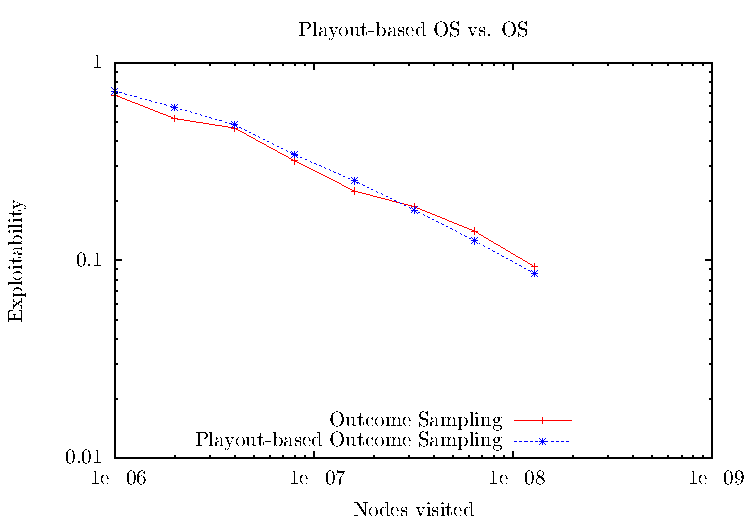
\includegraphics[scale=0.7]{figs/first-pbos/os-vs-pbos}
\caption{Preliminary convergence rate analysis of OS vs. playout-based OS. The vertical axis represents exploitability $\epsilon_{\bar{\sigma}}$.
\label{fig:os-vs-pbos}} 
\end{figure}

Playout-based OS seems to perform comparatively to OS in one domain. However, playout-based OS is not (yet) a search algorithm, 
since it does not take into account he current match history $\tth$. 
The main difficulty will be deciding how to direct the search when it is invoked {\it during the match}, \ie when the match 
history $\tth \not= \emptyset$. 

Online Outcome Sampling builds on playout-based OS by proposing several different ways to direct the search when started from a particular
match history, $\tth$. 

\subsection{Information Set Targeting}

Suppose the match history is $\tth$. Information set targeting OOS is playout-based OS that samples terminal histories $z \in Z_{I(\tth)}$ 
with higher probability than $z' \in Z - Z_{I(\tth)}$. The intuition is that these histories are particulary relevant since the searching player 
{\it knows} that one of these $z$ will describe the match at its completion. Let $\delta_I$ be the probability that any $z \in Z_{I(\tth)}$. 
Setting $\delta = 1$ is problematic, since convergence guarantees are lost. It is tempting to set $\delta_I$ high. 
The problem, however, is that 
focusing too much on $Z_{I(\tth)}$ could have the effect of revealing private information to the opponent. To see this, imagine the subgame 
defined by placing a single chance node over the histories $h \in I(\tth)$, whose distribution is obtained by previous chance event outcomes. 
The equilibrium strategy for the opponent in this subgame plays as if the opponent knows the searching player's private information. Therefore,
we expect that the optimal value of $\delta_I$ will depend on the importance of the hidden information.

\subsection{Public Subgame Targeting}

A \defword{public action}, $a \in A(I)$, to be one where for all $h \in I$, $ha \in I'$. (Need to define this better, i.e. include chance) 
Given a history $h$, let $p(h)$ be the sequence of public actions along $h$ in the same order that they were taken in $h$. 
Define the \defword{public subgame induced by h} to be the one whose terminal history set is
\[Z_{p,I} = \{ z | z \in Z, h \in I, h' \in H, p(h') = p(h), h' \sqsubset z \}\]
(Note that this is not a true subgame in the game-theoretic sense.)
Now, suppose the match history is $\tth$.
Public subgame targeting samples $z \in Z_{p,I(\tth)}$ with higher probability than terminal histories outside this set. 
Suppose $\delta_{p,\tth}$ is the probability that any $z$ in this set is sampled. 
Again, it is tempting to sample from this set with $\delta_{p,\tth} = 1$. 
However, this is also problematic because the probabilities to reach $\tth$ play a critical role in the convergence in the full game. 
Nonetheless, the intuition is to spend more time in parts of the tree that are relevant given the progression of the match. Unlike 
information set targeting, public subgame targeting should not reveal anything about private information. 

\section{Empirical Evaluation}

Here are some ides for what we could look at empirically: 

\begin{itemize}
\item Compare sampling techniques in each domain
\item Quality of OOS as a function of the length of the match history $\tth$ (and time limits?)
\item Robustness/sensitivity of $\delta_I$ and $\delta_{I,\tth}$ with observed convergence,
\item Importance of ``retaining the tree'' from previous searches along the same match $z$ (suspected to be high)
\item Performance comparisons (win rates and exploitability) between sampling techniques and some state-of-the-art
algorithms in imperfect information search (ISMCTS, PIMC, MMCTS), 
possibly also show exploitation / exploitability tradeoffs as in RNash work
\item (probably too much for this one paper) What if there are a sequence of multiple matches and we can reuse stuff from before?
\end{itemize}


\section{Conclusion}

\bibliographystyle{aaai}
\bibliography{iioos}

\end{document}
